\documentclass{article}
\usepackage[colorlinks]{hyperref}
\usepackage{pgfplots}
\usepackage{parskip}
\usepackage{subcaption}
\usepackage{minted}
\usepackage{mdframed}
\usepackage{color}
\usepackage{verbatim}
\usepackage[
  hmargin={1.3in,1.3in},
  vmargin={1in,1in},
  includefoot,
  footskip=30pt,
]{geometry}

\pgfplotsset{compat=1.13}

\pgfplotsset{every axis legend/.append style={legend pos=outer north east, font=\footnotesize}} 

\newcounter{codecounter}

\newcommand{\mycode}[4]{
  \vspace{1em}
  \begin{mdframed}[backgroundcolor=DarkGray, topline=false,bottomline=false,leftline=false,rightline=false]
  \refstepcounter{codecounter}Algorithm \thecodecounter: #2 \label{#1}
  \end{mdframed}
  \begin{mdframed}[backgroundcolor=LightGray, topline=false, bottomline=false, leftline=false, rightline=false]
    \inputminted
    [
      baselinestretch = 1.2,
      %fontsize        = \footnotesize,
      linenos,
      mathescape  = true,
      firstnumber = 1,
      fontsize=\small
    ]{#4}{#3}
  \end{mdframed}
  \begin{mdframed}[backgroundcolor=DarkGray, topline=false,bottomline=false,leftline=false,rightline=false]
  Algorithm \thecodecounter: #2
  \end{mdframed}
  \vspace{1em}
}

\usepackage{xcolor}
\definecolor{DarkGray}{gray}{0.7}
\definecolor{formalshade}{rgb}{0.95,0.95,1}
\definecolor{darkblue}{rgb}{0.21,0.24,59}
\definecolor{LightGray}{gray}{0.95}

\title{CS 267: Homework 3}
\author{Richard Barnes, Danny Broberg, Jiayuan Chen}
\date{April 5, 2016}

\hypersetup{
  pdfauthor={Richard Barnes, Danny Broberg, Jiayuan Chen},
  pdftitle={CS 267: Homework 3},
  pdfproducer={LaTeX},
  pdfcreator={pdfLaTeX}
}

\begin{document}
\maketitle

\section{Introduction}
This report describes our implementation of a de novo genome DNA assembly program using Unified Parallel C (UPC). UPC is an extension of the C language, outfitted for a Partitioned Global Address Space (PGAS) programming model. This model associates memory physically with specific processes but enables shared access. This bears syntatic similarities to OpenMP and other shared memory programming models.

Our paper is organized as follows:
\begin{enumerate} %TODO: Rewrite
\item description of the computational resources
\item a section that describes the general serial algorithm approach
\item a section that describes the general extension to UPC
\item evaluation of the code's performance
\end{enumerate}

\section{Machine Description}
For our codes we use NERSC's Edison machine. The machine has 5,576 compute nodes. Each node has 64GB DDR3 1866\,MHz RAM and two sockets, each of which is populated with a 12-core Intel ``Ivy Bridge" processor running at 2.4\,GHz. Each core has one or two user threads, a 256 bit vector unit, and is nominally capable of 19.2 Gflops. Notably, for our purposes, each core has its own L1 and L2 cache. The L1 cache has 64\,KB (32\,KB instruction cache, 32\,KB data) and the L2 cache has 256\,KB. The 12 cores collectively share a 30\,MB L3 cache. The caches have a bandwidth of 100, 40, and 23 Gbyte/s, respectively.\footnote{\url{http://www.nersc.gov/users/computational-systems/edison/configuration/}} Both the L1 and L2 caches are 8-way and have a 64 byte line size.\footnote{\url{http://www.7-cpu.com/cpu/IvyBridge.html}} 


\section{The Algorithm}
Sequencing long strands of DNA is difficult and time-consuming. For strands beyond a certain length it may not even be technically feasible. Therefore, faster and more scalable methods have been developed. Shotgun de novo genome assembly breaks a long piece of DNA into many shorter segments. These segments can be easily sequenced.

The problem then is to reassemble the original DNA by fitting the pieces together. In the simplified data set given here, the data takes the form of contiguous sequences of 19 or 51 bases (henceforth, a ``kmer") with known prefixes and suffixes. We are guaranteed that each kmer is unique. Together, the kmers a De Bruijn Graph.

Our program will construct this graph and traverse its connected components. To do this, a hash table will be used to store nodes of the graph with hashed kmers acting as keys. The values of the hash table will correspond to the prefix and suffixes and, thereby, serve as edges linking the nodes together.

Our algorithm begins by detecting how many kmers are in the input. It then allocates a shared memory hashtable three times larger than this number. Members of the hashtable are stored via open addressing with linear probing: this is wasteful of memory, but greatly simplifies the data structure, thereby reducing the potential for errors. Using a hashtable of size $3N$ ensures that occupancy stays well below 70\%, a point at which performance has been empirically shown to degrade significantly.

Kmers are hashed using Dan Bernstein's \texttt{djb2} hash function. Tests using the small data set with Austin Appleby's \texttt{MurmurHash3} didn't show a significant reduction in collisions.

Additionally, a local array of pointers to the hash table is allocated to be 1/50th the number of kmers. As the process reads kmers and adds them to the hash table, it makes a note of which kmers have prefixes indicating that they begin sequences and uses this local array to store that information. These starting-kmers (smers) form the starting points of the graph traversals which generated the contiguous (output) sequences. One might worry that storing smers locally would result in them being unevenly distributed; however, this is not a problem if we assume (a)~that the smers are distributed evenly throughout the file and (b)~that the smers, on average, are part of components of approximately equal size. These assumptions are reasonable because it is possible to randomize the order of the lines in the input file, which means that smers are evenly distributed and, therefore, component sizes should therefore be as well. For the purposes of the assignment, we do not randomize the input, but do verify that the assumption is at least nominally fulfilled by the test data provided.



  % int bucket_size = 3*line_count/THREADS;
  % hashtable_size  = bucket_size*THREADS;
  % smers_size      = line_count/50/THREADS;
  % kmers           = upc_all_alloc(THREADS, bucket_size*sizeof(kmer));
  % smers           = (kmer_ptr*) calloc(line_count/100/THREADS, sizeof(kmer_ptr));



\begin{comment}
Before coding up the genome assembly in parallel, we will first describe the approach for shotgun de novo genome assembly with a serial algorithm for comparison with setting up a UPC algorithm. Algorithm~\ref{serial} shows a cleaned up version of the main bulk of the code while Algorithms~\ref{packingDNAseq}--~\ref{contig_generation} show the code used to define packing routines and structures for the kmers. Overall one can see that there are three parts to the code: (1) Initialization of kmer values and hash table memory, (2) De Bruijn Graph Construction, (3) De Bruijn Graph Traversal. 

The code takes the input to be a set of unique k-mers along with their corresponding forward and backward extensions. To denote start/terminating kmer for a contig, there is a possibility of an extension being a ``guard" extension F which is incorporated into the hash table. We assume that the unique kmers have already been screened for errors so that the first step of the algorithm is to read in the unique values and construct a hash table with keys equal to the kmer and values equal to the forward and backward extensions. As shown in Algorithm~\ref{serial} the hash table is initialized with pre-allocated memory.  Within the graph construction step, the hash table is populated and a Start list is created to denote which Kmers will begin a contig. 

After the hash table has been populated, the Graph Traversal step begins by looping through the kmer Start list, which provides a ``seed" for the contigs that are created. Each traversal seed is added onto by appending the  the forward extension to the last n-1 k-mer values (where n is the kmer length defined in ~\ref{contig_generation}) and referring to the hash table for the next forward extension. This process is continued until a ``guard" extension is reached, at which point the contig is finished and printed to an external file. 

Within the serial code, many external functions and variables are referenced which were defined in Algorithms~\ref{packingDNAseq}- ~\ref{contig_generation}. These are displayed below the serial implementation code.
\end{comment}

\begin{table}
    \begin{tabular}[t]{|c|p{3.2cm}|}
        \hline
        &Alg. ~\ref{packingDNAseq} (packing sequences)\\ \hline
        1&\emph{Function} for initial lookup of kmers \\ \hline
        2&\emph{Function} to convert FourMer to packed\\ \hline
        3&\emph{Function} to pack sequences \\ \hline   
        4&\emph{Function} to unpack sequences \\ \hline
        5&\emph{Function} to compare packed sequences \\ \hline   
    \end{tabular}
    \hfill
    \begin{tabular}[t]{|c|p{3.2cm}|}
        \hline
        &Alg. ~\ref{kmer_hash} (kmer hashing)\\ \hline
        1&\emph{Function} to create hash table and pre-allocate memory\\ \hline
        2&\emph{Function} to compute hash sequence values \\ \hline
        3&\emph{Function} to return hash value of a kmer \\ \hline   
        4&\emph{Function} to look up Kmer and return a pointer to it\\ \hline
        5&\emph{Function} to add a kmer to hash table\\ \hline   
        6&\emph{Function} to add a kmer to start list  \\ \hline     
        7&\emph{Function} to deallocate memory buffers\\ \hline     
        8&\emph{Function} to deallocate hash table memory\\ \hline     
    \end{tabular}
    \hfill
    \begin{tabular}[t]{|c|p{3.2cm}|}
        \hline
        &Algorithm ~\ref{contig_generation} (contig generation) \\ \hline
        1&\emph{Function} for time keeping\\ \hline
        2&\emph{Structure} for Kmer data \\ \hline
        3&\emph{Structure} for start-kmer \\ \hline   
        4&\emph{Structure} for buckets\\ \hline
        5&\emph{Structure} for hash table \\ \hline   
        6&\emph{Structure} for working memory buffers\\ \hline   
        7&\emph{Function} for getting number of Kmers in file \\ \hline   
    \end{tabular}
    \caption{Functions and Structures included in Algotithms~\ref{packingDNAseq}- ~\ref{contig_generation}}
\end{table}

%\mycode{serial}{Serial Implementation (C)}{code-serial.c}{c} 

%\mycode{packingDNAseq}{DNA packing routine (Fortran)}{code-packingDNAseq.h}{fortran}

%\mycode{kmer_hash}{k-mer hash table routine (Fortran)}{code-kmer_hash.h}{fortran}

%\mycode{contig_generation}{Generation of contigs routine (Fortran)}{code-contig_generation.h}{fortran}



\section{UPC approach}
The first thing to be done in the extension to UPC was to rewrite the packing and hashing functions for a PGAS framework. This gives us an initial list of start kmers ({\color{red}Elaborate on changes for these functions}). 

Next a function was built for finding the next kmer, so that graph traversal can occur in the partition global address space. This allows one to get to the point of allowing contigs to be generated({\color{red}Elaborate on changes for this function}).

At this point a choice needed to be made for the communication of PGAS threads. We decided to read input into a circular buffer that all the threads could then have blocks of dedicated address space in. ({\color{red}insert better explanation of how this buffer works?})

Later we considered the option of enabling parallel read-in capabilties, since at this point the UPC code did a sequential read in and then distributed the input accross the partitioned global memory space. This means that the only benefit from using PGAS came from having access to a large memory space, but no improvements in speed could be gained yet. 

 To perform a parallel read-in, we hoped to involve atomics on the hash table - and we consider the use of conditional swap as a method for implementing this. However, atomic procedures are not traditionally used for individual bytes and we were not able to find a Berkeley UPC atomics library. We therefore considered using UPC locks instead - which has it's own difficulties due to the inability to lock an openly addressed hash table. As an alternative strategy we decided to partition the table into blocks of 100 do locking on the individual blocks. ({\color{red}Insert code to describe how this works}) 

 This methodology works only if the probability of a lock collision is relatively small. ({\color{red}Insert part about the relative probability of collisions existing for certain hash tables... ?}) 

%stuff about number of collisions existing for different types of hash tables (amount of randomness)?
%sequence starting kmers are distributed fairly evenly throughout the test file
%more stuff about randomness of kmers being distributed being important for load balancing? In real life it is possible to randomize the line order of the file...but this means each processor can keep track of its starting-mers locally

After testing the code further at this point, numerous deadlocks were witnessed. To address this issue, we decided to try synchronized rotating access to chunks of the table - which resulted in an intiial code that was faster than the serial version. ({\color{red}Insert a figure comparing initial performance against serial version?})

In the later stages of the code, local representations of the hash tables were created to avoid synchornization issues. We also began to wonder if things could be  made faster with linked lists, which would have $\circ (1)$ insertion time and $\circ(BinN)$ retrieval time, as opposed to open hash table approaches which have $\circ (BinN)$ for both. If the circular buffer method was still applied to linked lists, then the approach could remain lock free. 

\begin{minipage}{\linewidth}
  \captionsetup{type=figure}
  \begin{center}
  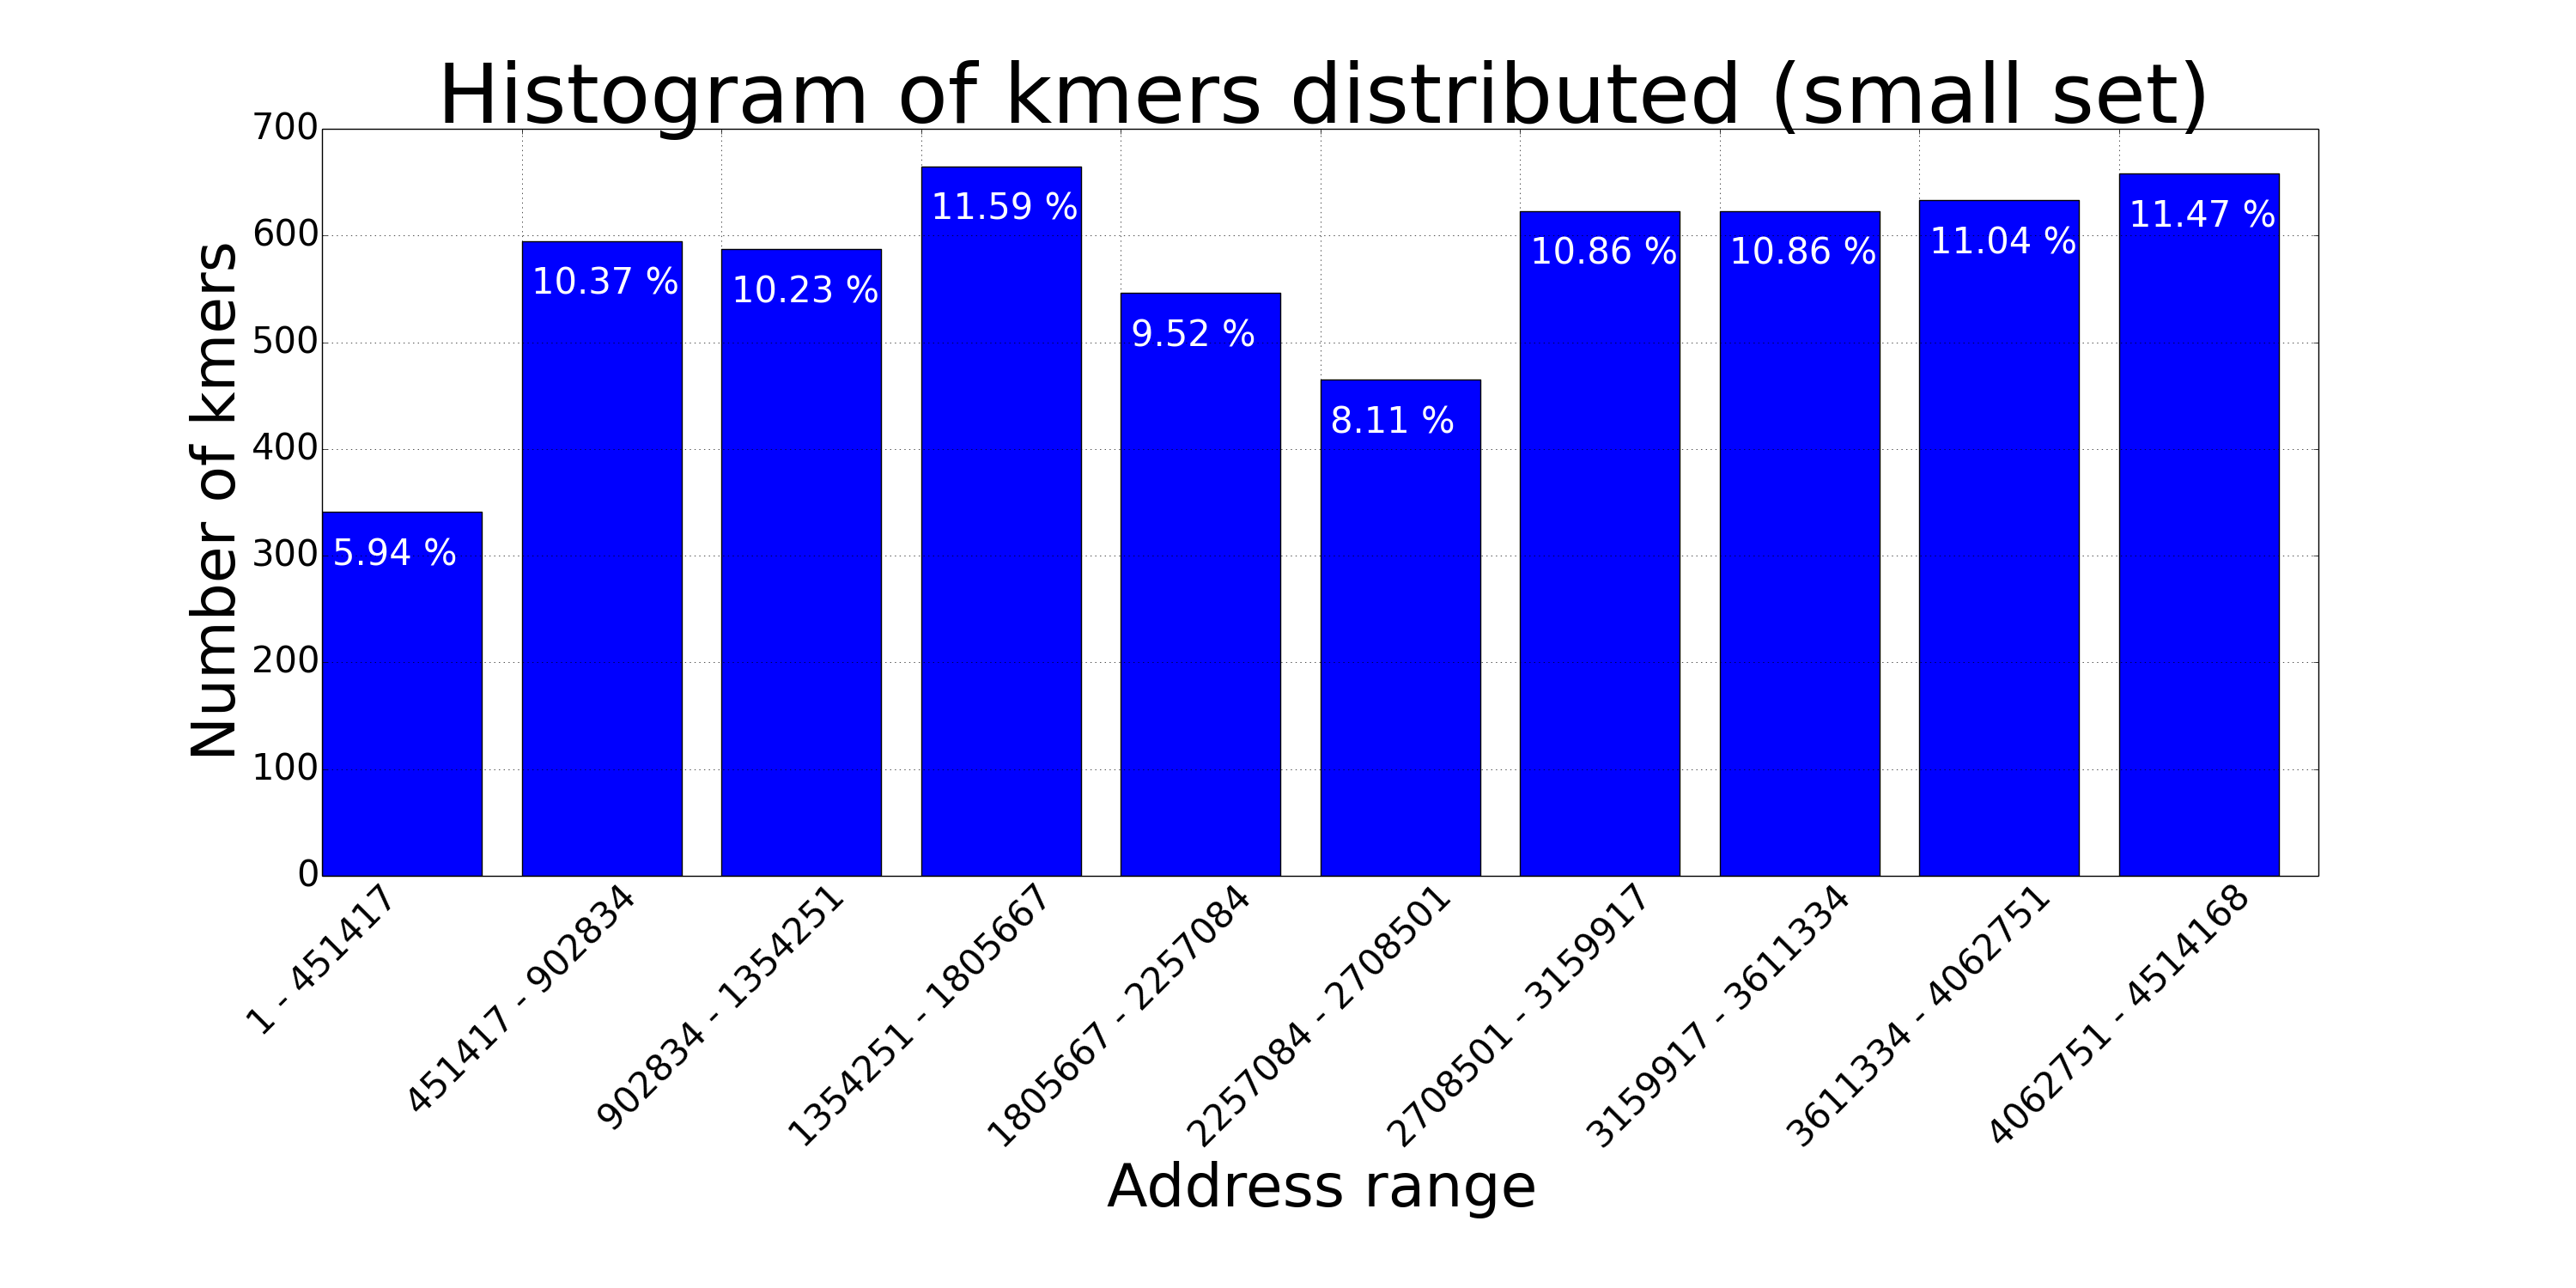
\includegraphics[width=0.5\textwidth]{shorthisto.png}
  \end{center}
  \caption{Distribution of start kmers to address space (Short data set)} \label{fig:xsl_script}
\end{minipage}

\begin{minipage}{\linewidth}
  \captionsetup{type=figure}
  \begin{center}
  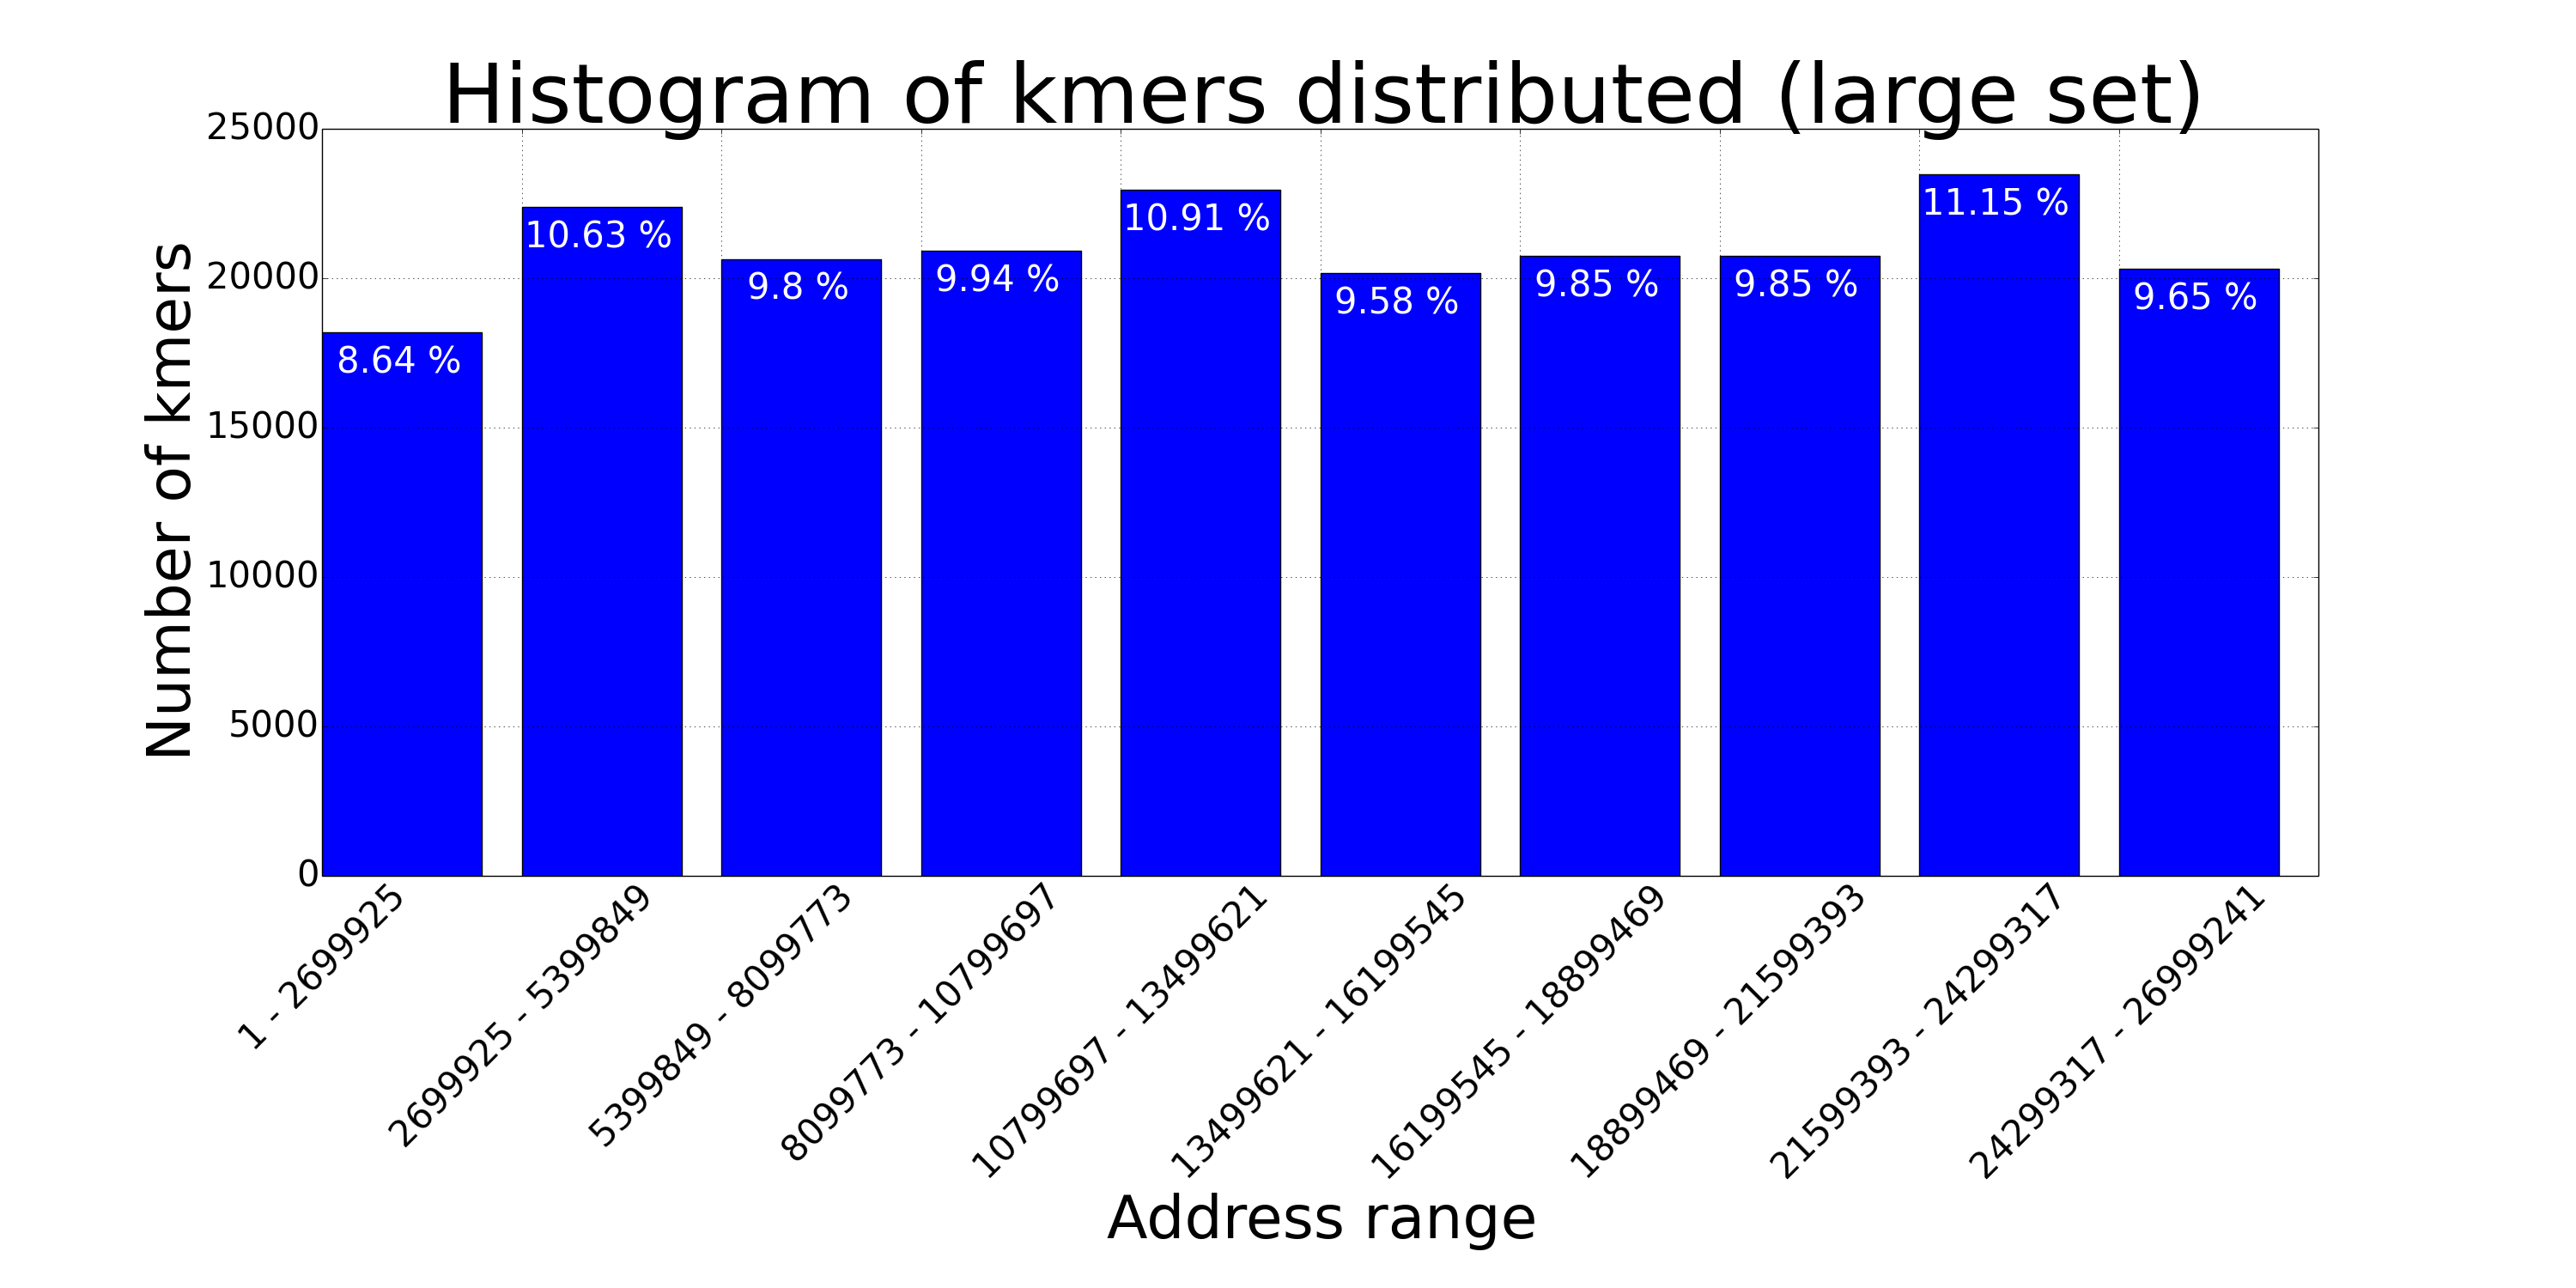
\includegraphics[width=0.5\textwidth]{longhisto.png}
  \end{center}
  \caption{Distribution of start kmers to address space (Long data set)} \label{fig:xsl_script}
\end{minipage}


figures/plots that could exist:
\begin{itemize}
\item distribution of large and small k-mer test set distributions
\end{itemize}

List of suggested thigns to include from homework statement:
\begin{itemize}
\item A description of your distributed data structures and parallel algorithms
\item A description of the computational and communication motifs of the parallel algorithms.
\item A description of the design choices/optimizations that you tried and how did they affect the performance.
\item A description of how you avoided race conditions.
\item Speedup plots that show how closely your parallel code approaches the idealized p-times speedup in the two experimental scenarios described in the previous section.
\item Discussion of the scalability and relative costs of the parallel graph construction and traversal algorithms.
\item A discussion on using UPC for such an application with the underlying computational motif.
\item A discussion on how would you implement the same parallel algorithms in a two-sided communication model (e.g. by using MPI).
\end{itemize}

\section{Performance}
\begin{itemize}
\item Simple compared results against serial implementation.
\end{itemize}

\section{Summary}


\end{document}
